\chapter{RESEARCH METHODOLOGY}

\section{Introduction}
This chapter will be discussed about the methodology for evaluating Japanese ASR on three pre-trained speech recognition model that is OpenAI’s Whisper, Meta’s wav2vec 2.0, and Google’s CHIRP (USM). This study will be focusing on comparing the Word Error Rate (WER) and transcription speed using formal (TED Talks) and informal (dialectal, COJADS) datasets. In this chapter, the data collection and data pre-processing steps such as audio conversion and resampling will be discussed. This chapter also will be discussing about the reason why the three model is selected and also the standardized testing environment. It concludes by discussing challenges, limitations, and ethical considerations relevant to the evaluation process.

\section{Research Design}
This study is conducted in four phase that is Preparation, Data Collection, Analysis, and Discussion. The details for each phase is described in the Table \ref{tab:methodology_plan} below.

\begin{table}[H]
    \centering
    \caption{Overview of the Research Methodology Plan}
    \label{tab:methodology_plan}

    \begin{tabular}{ p{2cm}|p{4cm}|p{4cm}|p{4cm} }
    \hline
    \textbf{Phases} & \textbf{Activity} & \textbf{Methods} & \textbf{Deliverables} \\
    \hline
    \hline
    
    \textbf{Phase 1 -- Preparation}
     & i. Define Area 
       \newline ii. Define Problem Statement
       \newline iii. Define Research Objectives, Scope, Questions, and Significance
     & i. Review related articles and journals
       \newline ii. Discussion with supervisor
     & Research Proposal \newline \& Chapter 1 \\
    \hline
    
    \textbf{Phase 2 -- Data Collection} 
     & i. Study in detail the articles on the area of Speech Recognition
       \newline ii. Identify challenges in Japanese ASR
       \newline iii. Identify the most efficient techniques for improving WER and transcription latency
     & i. Literature Review
       \newline ii. Data collection method:
        \newline \hspace*{1em}a) TED Talks YouTube dataset
        \newline \hspace*{1em}b) COJADS dataset
        \newline iii. Data preprocessing
     & i. Target model selection
        \newline ii. Processed audio files
        \newline iii. Test environment setup \\
    \hline
    
    \end{tabular}
    \hfill
    \begin{tabular}{ p{2cm}|p{4cm}|p{4cm}|p{4cm} }
    
    \textbf{Phase 3 -- Analysis} 
        & i. Evaluate the performance of the selected models
        \newline ii. Calculate WER and transcription latency
        \newline iii. Compare the models based on the evaluation metrics
        & i. Model testing and evaluation
        \newline ii. Performance metrics calculation
        & i. Performance comparison results
          \newline ii. Analysis of the models' strengths and limitations \\
    \hline

    \textbf{Phase 4 -- Discussion} 
        & i. Identify challenges and limitations
        \newline ii. Summarize the research findings
        & i. Challenges and limitations identification
        \newline ii. Research findings summary
        & i. Dissertation research report \\
    \hline
    
    \end{tabular}
\end{table}


\section{Data Collection}
\subsection{Dataset Selection}
To evaluate the performance of the models, this study will be using two sources of data. The first dataset is from Ted Talk Youtube dataset which will be responsible for formal speech with clear pronunciation completes with rich and diverse vocabulary. The second dataset is the Corpus of Japanese Dialects (COJADS) which will be responsible as the input for informal speech which categorized based on regional accent and expression. The COJADS dataset only can be obtain from National Institute for Japanese Language and Linguistics (NINJAL). Both of the dataset duration will be around 6 hours where duration for COJADS will be 1 hours for each dialect sum up to 6 hours for dialectical speech. The duration of the dataset can be seen in Table \ref{tab:dataset_length}.

\begin{table}[H]
    \centering
    \caption{Dataset Audio Duration}
    \label{tab:dataset_length}
    \begin{tabular}{p{3.5cm}|p{2.5cm}|p{2cm}}
    \hline
    \textbf{Dataset} & \textbf{Dialect} & \textbf{Duration} \\
    \hline
    TED Talks (YouTube) & Formal & 6 hours \\
    \hline
    \multirow{5}{*}{COJADS} 
        & Tōhoku & 1 hours \\
        & Kantō & 1 hours \\
        & Chūbu & 1 hours \\
        & Kansai & 1 hours \\
        & Shikoku & 1 hours \\
        & Okinawa & 1 hours \\
    \hline
    \multicolumn{2}{c|}{\textbf{Total}} & \textbf{12 hours} \\
    \hline
    \end{tabular}
\end{table}


\subsection{Data Pre-processing}
The pre-processing steps is the first step in doing the model comparison. This step will be focusing in preparing the datasets to be use as input into the selected speech recognition models. For the TED Talks YouTube dataset, the audio files will be extracted from video recordings and transcribed using Python Moviepy library into Waveform Audio File Format (WAV) format.
\begin{lstlisting}[caption={Python code to convert video to WAV format using moviepy}]
    def convert_video_to_wav(video_path, output_wav_path):
    try:
        video_clip = VideoFileClip(video_path)
        audio_path = output_wav_path\
            .replace(".wav", "_temp_audio.mp3")
        video_clip.audio.write_audiofile(audio_path)
        return audio_path
    
    except Exception as e:
        return None
\end{lstlisting}
After that, each audio file was converted to the standardized 16 kHz, 16-bit PCM format to ensure the data is compatible with the ASR models. Then the text will be manually transcribed and aligned with the corresponding audio to create accurate transcriptions for evaluation phase later.

For the COJADS dataset, the data is in MP4 format and the audio files will be extracted to wav using the same method as the TED Talks YouTube dataset. Then the audio files will be resampled to the 16 kHz, 16-bit PCM format using Pydub library from Python.

\begin{lstlisting}[caption={Python code to resample audio to 16 kHz using pydub}]
    def resample_audio(input_audio_path, output_audio_path,\
        target_sample_rate=16000):
    try:
        audio = AudioSegment.from_file(input_audio_path)
        audio = audio.set_frame_rate(target_sample_rate)
        audio.export(output_audio_path, format="wav")
        
        print(f"Resampled audio saved to {output_audio_path}")
    except Exception as e:
        print(f"Error during audio resampling: {e}")
\end{lstlisting}
The reason for resampling the audio into 16 kHz is that many modern ASR models are trained on and optimized for audio data sampled at this rate. By standardizing the sample rate, the input data compatibility with the expected model parameters can be ensured, thus helping to avoid potential performance issues due to mismatched sample rates or quality. Additionally, a 16 kHz sampling rate provides a good balance between audio quality and computational efficiency, making the ASR systems both accurate and faster to process. Image \ref{fig:resampling} shows audio before and after resampling.

\begin{figure}[H]
    \centering
    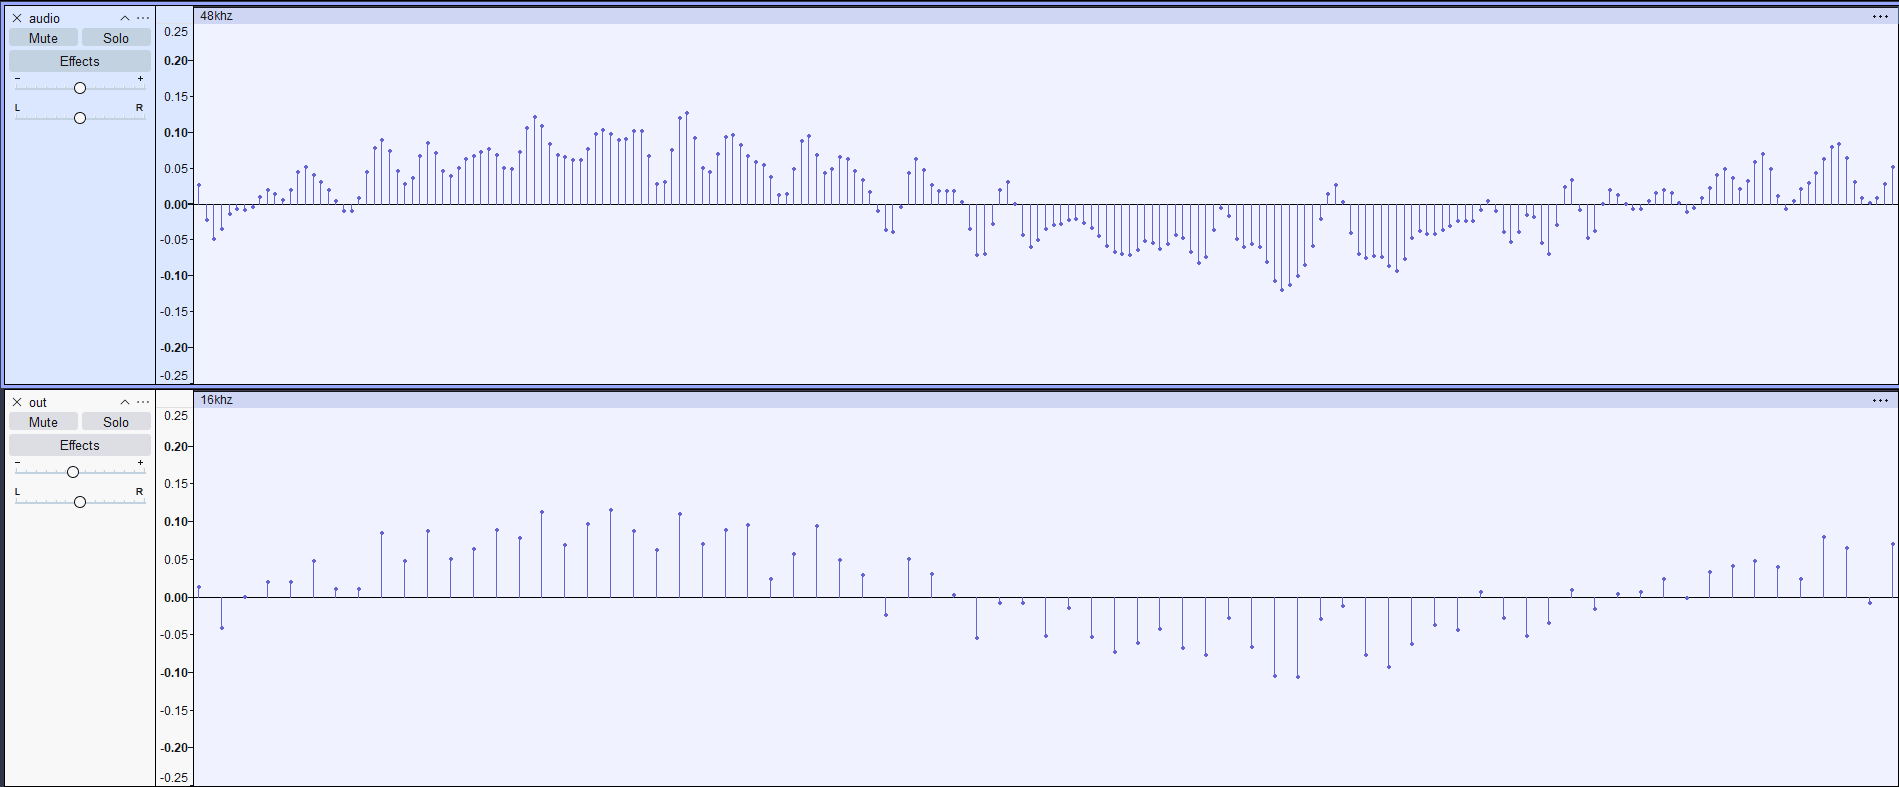
\includegraphics[width=1\textwidth]{mainmatter//images/bitrate.png}
    \caption{Audio resampling from 44.1 kHz(Top) to 16 kHz(Bottom)}
    \label{fig:resampling}
\end{figure}


\section{Model Selection}
To evaluate the best-performing model for Japanese speech recognition, this study focuses on three state-of-the-art models: Whisper by OpenAI, wav2vec 2.0 by Meta, and CHIRP (USM) by Google. These models are compared not only against each other but also with traditional and modern ASR approaches to justify their selection.

Comparative Analysis with Traditional and Modern ASR Models
Traditional Models
Gaussian Mixture Model-Hidden Markov Model (GMM-HMM):

Strengths: Well-established for speech recognition with the ability to model temporal variability in speech and complex acoustic features like pitch accents.
Weaknesses: Struggles with the scalability required for Japanese, given its syllable-based phonetic structure and dialectical variations. Lacks adaptability to informal speech and is computationally inefficient compared to modern models.
Hidden Markov Models (HMM):

Strengths: Effective for sequential data and capturing temporal dependencies, making it suitable for languages with rhythmic speech patterns like Japanese.
Weaknesses: Performance is constrained by the reliance on handcrafted features and limited discriminative power compared to deep learning models.
Modern Deep Learning-Based Models
Deep Neural Networks (DNN):

Strengths: Significantly improves recognition accuracy by leveraging large datasets and powerful feature extraction. DNN-HMM combinations outperform traditional models in Japanese ASR tasks.
Weaknesses: Limited in handling contextual dependencies and dialectical variations without substantial pretraining or fine-tuning.
Recurrent Neural Networks (RNN):

Strengths: Effective for modeling sequential data and addressing Japanese intonation and pitch accent issues. Bidirectional LSTMs (BLSTMs) achieve strong performance by using past and future contexts.
Weaknesses: Computational inefficiency and gradient-related issues, such as vanishing gradients, limit scalability.
Convolutional Neural Networks (CNN):

Strengths: Efficient in capturing acoustic patterns in spectrograms and time-frequency domain features.
Weaknesses: Limited contextual understanding for longer sequences, reducing effectiveness for Japanese dialects.
Transformer-Based Models:

Strengths: State-of-the-art performance in ASR due to their ability to process long sequences with attention mechanisms. Conformer models, in particular, outperform traditional and earlier neural network models in Japanese ASR tasks.
Weaknesses: Requires extensive computational resources for training.
Comparison with Chosen Models


Justification for Selection of Whisper, wav2vec 2.0, and CHIRP
Whisper:
Outperforms traditional and earlier modern approaches with its encoder-decoder Transformer architecture, optimized for multilingual transcription.
Addresses Japanese-specific challenges such as Kanji recognition and contextual syllables.

wav2vec 2.0:
Excels in low-resource settings and regional dialect transcription due to its self-supervised learning approach, outperforming traditional GMM-HMM and DNN-HMM models in accuracy and adaptability.

CHIRP (USM):
Scales to 300 languages using self-supervised and chunk-wise attention mechanisms, making it superior to traditional and RNN-based models for processing long audio sequences and diverse inputs.

\begin{table}[ht]
    \centering
    \caption{Comparison of Traditional, Modern, and Chosen ASR Models}
    \begin{tabular}{p{2.5cm}|p{3.5cm}|p{3.5cm}|p{3.5cm}}
    \hline
    \textbf{Criteria} & \textbf{Traditional (GMM-HMM)} & \textbf{Modern (DNN, RNN, CNN)} & \textbf{Chosen Models} \\ \hline
    \textbf{Accuracy on Japanese} & Limited, struggles with dialects & Improved, handles linguistic features better & High, especially in informal and dialectical contexts \\ \hline
    \textbf{Scalability} & Low & Moderate & High, designed for multilingual and diverse inputs \\ \hline
    \textbf{Contextual Understanding} & Poor & Moderate to High & High, leveraging large-scale pretraining datasets \\ \hline
    \textbf{Adaptability to Dialects} & Low & Moderate & High, particularly with wav2vec 2.0 and CHIRP \\ \hline
    \textbf{Computational Efficiency} & Low & Moderate & Moderate to High (Whisper and CHIRP optimized) \\ \hline
    \end{tabular}
    \label{tab:comparison_models}
\end{table}

    
For this study, three models have been selected based on their state-of-the-art technology and performance in speech recognition. These models also has been selected based on their compatibility with the research objectives. The first selected model is Whisper from OpenAI for its ability to perform very well in multilingual and multitask environments using large-scale weak supervision \parencite{radford2023robust}. The architecture that based on simple encoder-decoder transformers has increase its performance transcription across various languages. The whisper model has been trained by using over 680,000 hours of audio. This makes it a very suitable model for addressing the issue of context-based syllable recognition and complex script systems in Japanese ASR \parencite{bajo2024efficient}. 
 
The second model that has been selected is Meta’s wav2vec 2.0. This model has been selected because of its innovative self-supervised learning approach where only small amount of labelled data is needed to train this model \parencite{baevski2020wav2vec}. It also has the ability to learn speech representations directly from raw audio, followed by fine-tuning on smaller labelled datasets, makes it particularly suitable for handling low-resource languages and diverse dialects. Because of that, wav2vec is very suitable to handle  regional dialects and informal speech  in Japanese language \parencite{miwa2023dialect}. 

The third selected model is CHIRP that build based on Universal Speech Model was chosen for its emphasis on multilingual scalability. This model has been trained on an extensive dataset encompassing 300 languages. Its BEST-RQ pretraining framework and innovative chunk-wise attention mechanism offer significant advantages in processing long audio sequences and handling diverse linguistic inputs \parencite{zhang2023google}. Its superior performance in low-resource languages positions it as a strong contender for addressing Japanese speech recognition challenges, including phonetic ambiguities and dialectical diversity.


\section{Model Testing and Evaluation}
\subsection{Testing Environment}
The model testing will be using the Hugging Face platform, which is a widely used and versatile framework for deploying and testing Machine Learning models. Hugging Face provides out of the box integration with the chosen speech recognition models. This is the example of the code to load and run the Whisper model from Hugging Face by using python pytorch and transformers library.

\begin{lstlisting}[caption={Python code to load Whisper model from Hugging Face}]
    import torch
    from transformers import pipeline

    whisper = pipeline("automatic-speech-recognition",\
        model="openai whisper-large-v3")
    transcription = whisper("Sample_audio.mp3",\
        chunk_length_s=30)
    print(transcription["text"][:500])
\end{lstlisting}

To provide better and more consistent evaluations, the testing environments for all models will be standardized. The sample will be prepared using the same preprocessed method for audio files which are sampled at 16 kHz and follow the 16 bit PCM standard. This will make sure all the input data will be compatible with the models then the test will be conducted in the same environment to provide identical hardware and software configurations, so the results of the models can be compared. 


\subsection{Performance Metrics}
To evaluate the performance of the selected speech recognition models, these key metrics will be used:

\begin{enumerate}
    \item Word Error Rate: Measures the accuracy of transcriptions by calculating the percentage of words that incorrectly transcribed. This is a critical metric for assessing the overall precision of the models.
    \[
    \text{WER} = \frac{S + I + D}{N} \times 100\%,
    \]
    where:
    \begin{itemize}
        \item \(S\) = Number of substitutions
        \item \(I\) = Number of insertions
        \item \(D\) = Number of deletions
        \item \(N\) = Total number of words in the \textbf{reference} transcription
    \end{itemize}

    \item Transcription Latency: Measures the time taken by each model to transcribe audio input, providing insight into their suitability for real-time applications.
    \[
    \text{Latency}_i = t_{\text{end}}(i) - t_{\text{start}}(i),
    \]
    where:
    \begin{itemize}
        \item \(t_{\text{start}}(i)\) = Timestamp when the model begins receiving or processing the \(i\)-th audio.
        \item \(t_{\text{end}}(i)\) = Timestamp when the final transcription for the \(i\)-th audio is produced.
    \end{itemize}

    To compute the average latency over \(M\) utterances:
    \[
    \text{Average Latency} = \frac{1}{M} \sum_{i=1}^{M} \left( t_{\text{end}}(i) - t_{\text{start}}(i) \right).
    \]

    \item Handling of Formal vs. Informal Language: Evaluates how well the models perform across different linguistic contexts, including formal speech and informal, dialectal speech.
    \[
    \text{WER}_{\text{informal}} = \frac{S_i + I_i + D_i}{N_i} \times 100\%,
    \]
    where:
    \begin{itemize}
        \item \(S_i, I_i, D_i\) = Substitutions, insertions, and deletions within the informal subset.
        \item \(N_i\) = Total number of reference words in the informal subset.
    \end{itemize}
\end{enumerate}

\subsection{Test Procedure}
The following step-by-step procedure was implemented to evaluate the models:

\begin{figure}[!ht]
    \centering
    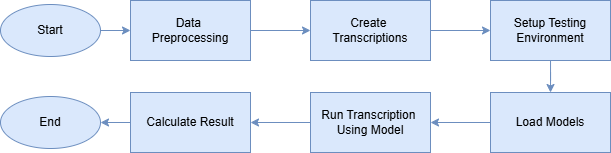
\includegraphics[width=1\textwidth]{mainmatter//images/step.png}
    \caption{Testing procedure }
\end{figure}

In order to make sure the audio input file to be consistence across the dataset, the model evaluation will be start by pre-processing all the input data. This will make sure that the input data is compatible with the targeted models. Then, the pre-processed data that did not have transcription ready will be transcribe manually. These data is usually come from Ted Talk Youtube dataset because all data from COJADS has its transcription ready.

After the input data is ready, the preparation for testing environment will be carried out. The testing environment will be using model that prepared by Hugging Face as the platform comes with controlled configuration. Then the selected model will be load from the Hugging Face platform input data will be fed into the models one by one automatically. After that, the output transcription will be compared with the benchmark transcription to evaluate the accuracy metric and to observe each model ability. 

\section{Challenges and Limitations}
One of the major challenges in this study is the availability of high quality dataset that has comes with annotation for Japanese speech recognition. Although the dataset like TED Talks YouTube and the Corpus of COJADS gives a valuable resources, they may not fully cover all the different aspect in the linguistic diversity in Japanese. Not only that, the variations in recording quality and noise levels within the datasets may also introduce inconsistencies that may affect the models’ performance evaluation.

Another limitation during carried out this study is the bias that may be occur during the dataset selection process. Dataset from Ted Talk Youtube may only capture the formal Japanese language without having enough representation for daily use of the Japanese language. The Corpus of COJADS dataset also may only be capture the six most major dialects in Japanese while ignoring other dialects as there is not enough data available to be used in this test. Because of this bias, it could temper the evaluation results by favoring models better suited to the specific characteristics of the datasets. 

\section{Ethical Considerations}  
In this study, the ethical challenges that may be rise is on data privacy, consent and the fairness when evaluating the models. The dataset that has been used in the study contain publicly available speech recordings and there is no private or sensitive information is disclosed. Apart from that, the dataset from Ted Talk Youtube and the COJADS is widely available and can be obtain easily thus did not require individual consent for research purposes. This study will only be using the data for evaluating the performance of speech recognition models rather than analyzing the content of the recordings, reducing potential privacy concerns.

\section{Summary}
In this chapter, a clear research design was laid out to compare three ASR models on Japanese speech. Formal (TED Talks) and informal (COJADS) datasets were chosen for linguistic variety, and consistent preprocessing steps were described. The reasoning for selecting Whisper, wav2vec 2.0, and CHIRP (USM) was explained, followed by details on how testing will be conducted in a standardized environment to measure WER and transcription latency. Lastly, challenges in dataset availability, biases, and ethical considerations around data privacy were also addressed in this chapter.